\documentclass{beamer}
\usepackage{etoolbox}\newtoggle{printable}\togglefalse{printable}
\usetheme{default}
\usecolortheme{beaver}
\usepackage{listings}
\usepackage{algpseudocode}
\graphicspath{ {./images/} }
\pdfmapfile{+sansmathaccent.map}


\title{Comp320 Research Artifact}
\author{Alastair Rayner}
\date{\today}

\begin{document}

\maketitle


\begin{frame}{Research Questions}
	\textbf{My Research questions I aim to answer}
	
	%Old
	%\begin{itemize}
    	%	\item How does game tree search techniques compare for GVGAI? \pause
    	%	\item Where does each tree search technique do well in each game? \pause 
    	%	\item What are the strengths and weaknesses of different search techniques and how can they be improved? \pause
	%\end{itemize}
	
	%New
	\begin{itemize}
		\item Can visualizing the actions an agent may take in the competition lead to insights about the strengths and weakeness of each tree search algorithm \pause
		\item How can the scaling of different metrics within the competition affect the performance of different tree search algorithms \pause
		\item Could a hyper-heuristic be created from the strengths of multiple tree search algorithms
	\end{itemize}
\end{frame}



%How will this contribute to knowledge in the field
\begin{frame}{The Goal of this Research Artifact}
		\textbf{The Goal} \pause
		\begin{itemize}
			\item To create a hyper heuristic agent that has been modified from the strengths and weaknesses found in different tree search techniques. \pause
			\item The strengths and weaknesses will be found by visualizing and analyzing the search space of a tree search algorithm.   \pause
			\item Also by looking at how the scaling of different metrics within the competition frame work and seeing how they affect the performance of different agents.
		\end{itemize}
\end{frame}


% What have I obtained so far
\begin{frame}{Preliminary results}
\textbf{Visualizations for the GVG-AI Competition}
		\begin{itemize}
			\item One of my main focuses this far is to get visualizations rendering over the competition. \pause
			\item This will help facilitate the data collection about the strengths and weaknesses of different search algorithms. \pause
			\item Being able to visualize where the agent is planning to go and finds most interesting/valuable to explore can help to creating an hyper heuristic \pause
		\end{itemize}
		
		\begin{itemize}
			\item An example of the different metrics that can be tweaked to see how they affect the agents success rate are: \pause
			\item Competition time \pause
			\item MCTS iterations \& Exploration vs Exploitation ratio, and other tree search equivalents 
		\end{itemize}
\end{frame}

\begin{frame}{The Next Step}
\textbf{The Next Step}
		\begin{itemize}
			\item Finish the visualizations of the different tree search algorithms \pause
			\item Gather the data about where different tree search techniques succeed and what are their limitations \pause
			\item Use that data to start creating a hyper-heuristic agent that can take advantage of different tree search strengths \pause
			\item Submit that agent to the GVG-AI competition
		\end{itemize}
\end{frame}

\begin{frame}{Demo of the GVG-AI competition}
		\textbf{Example Games}
		\begin{figure}[t]
				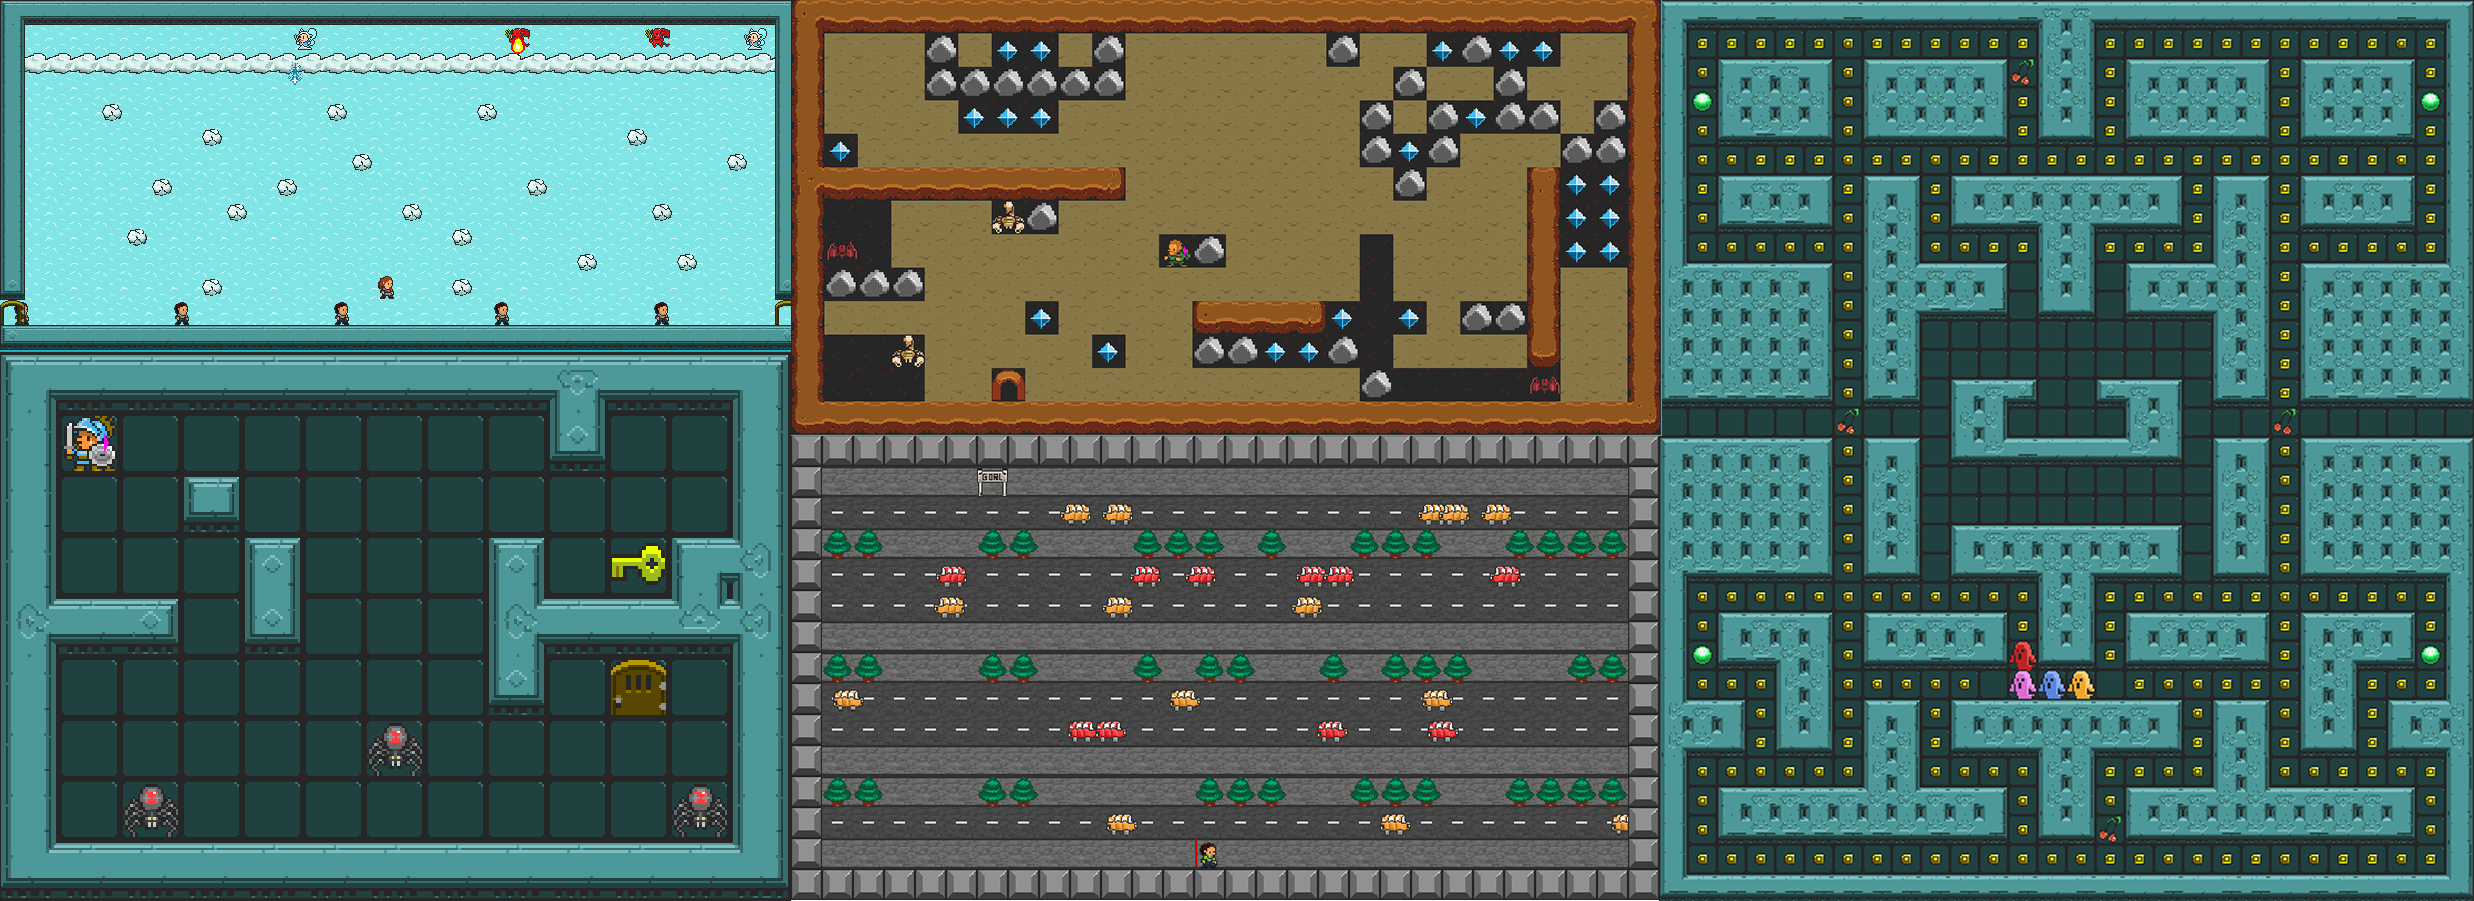
\includegraphics[width=10cm]{VGDL}
		\end{figure} 
		Angles, BoulderDash, Pac-man, Zelda, Frogger.
		
\end{frame}

\begin{frame}{Demo of the GVG-AI visualizations}
		\textbf{Example of MCTS visualisations}
		\begin{figure}[t]
				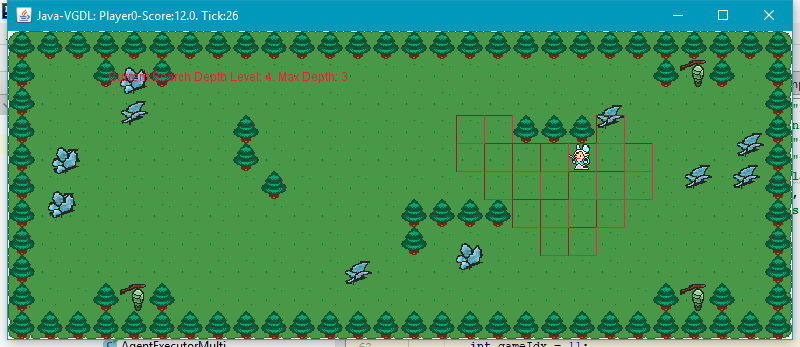
\includegraphics[width=5cm]{Game-51-5}
				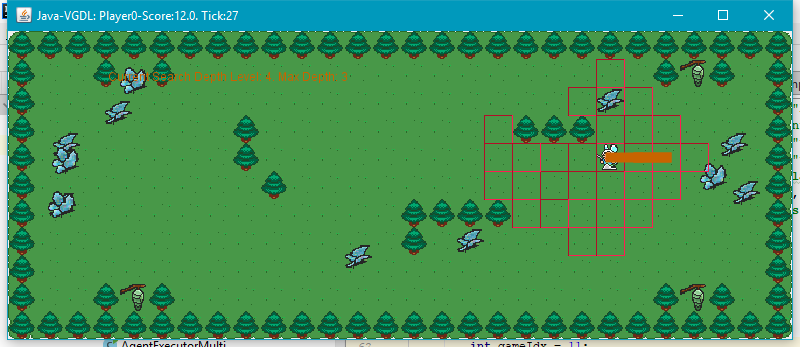
\includegraphics[width=5cm]{Game-51-6}
				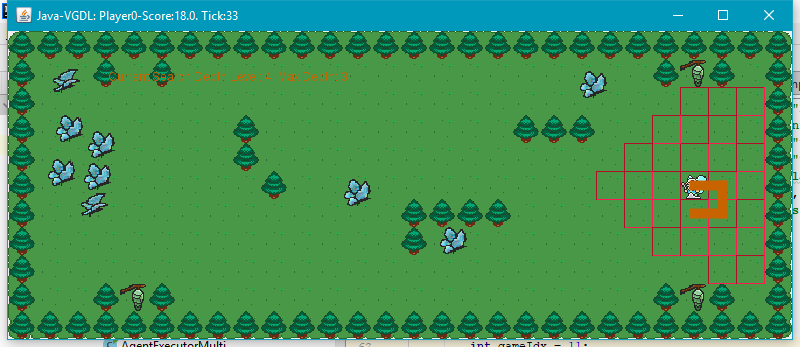
\includegraphics[width=8cm]{Game-51-7}
		\end{figure} 
\end{frame}

\begin{frame}{Demo of the GVG-AI competition and visualizations}
\center
		\textbf{Live Demo!}
\end{frame}


\begin{frame}{Questions?}
\center
		\textbf{Questions?}
\end{frame}



\end{document}
